%! Author = christophherb


\documentclass[a4paper, 12pt]{article}
%TC:incbib

%%%%%%%% CREATE DOCUMENT STRUCTURE %%%%%%%%
%% Language and font encodings
\renewcommand*{\familydefault}{\sfdefault}
\usepackage[ngerman]{babel}
\usepackage[utf8]{inputenc}
\usepackage[T1]{fontenc}
\usepackage{microtype}% verbesserter Randausgleichjk
\usepackage[scaled]{uarial}
%\usepackage{subfig}

%% Sets page size and margins
\usepackage[a4paper,top=3cm,bottom=2cm,left=2cm,right=2cm,marginparwidth=1.75cm]{geometry}

%% Packages
\usepackage{amsmath}
\usepackage{graphicx}
\usepackage[colorlinks=true, allcolors=black]{hyperref}
\usepackage{caption}
\usepackage{subcaption}
\usepackage{sectsty}
\usepackage{apacite}
\usepackage{float}
\usepackage{titling}
\usepackage{blindtext}
\usepackage[square,sort,comma,numbers]{natbib}
\usepackage[colorinlistoftodos]{todonotes}
\usepackage{xcolor}
\definecolor{darkgreen}{rgb}{0.0, 0.4, 0.0}
\definecolor{LightGray}{gray}{0.8}
\usepackage{verbatim}
\usepackage{booktabs}
\usepackage{longtable}
\usepackage{pdfpages}

\setcounter{secnumdepth}{4}

%%%%%%%% Functions %%%%%%%%
%% Count Characters
\newcommand{\charactercount}[1]{
    \immediate\write18{
        expr `texcount -1 -sum -merge #1.tex` + `texcount -1 -sum -merge -char #1.tex` - 1
        > build/.chars.txt
    } 
    \input{build/.chars.txt}
}

%% Count Words
\newcommand{\quickwordcount}[1]{%
    \immediate\write18{
      texcount -1 -sum -merge -q #1.tex > build/.#1-words.sum 
    }
    \input{build/.#1-words.sum}%
}


%%%%%%%% Variables %%%%%%%%
\newcommand{\HRule}{\rule{\linewidth}{0.5mm}} 							% horizontal line and its thickness


%%%%%%%% DOCUMENT %%%%%%%%
%%%% Title Page
\begin{document}
    \begin{titlepage}
        \center
        %\vspace*{2.0cm}
        \includegraphics[width=0.45\textwidth]{../images/hsa_logo}\\[0.5cm] 	% University logo
        \includegraphics[width=0.3\textwidth]{../images/logo}\\[1.5cm] 	% University logo

        \HRule \\[0.2cm]
        {
          \huge \bfseries todo\\
          \large Dokumentation der Anwendung\\[0.5cm]
          \large Full-Stack-Webanwendungen\\
          \large Sommersemester 2023
        }\\[0.2cm]								% Assignment
        \HRule \\[2cm]

        \begin{flushleft}
          \large
          Lucas Schiessl\\
          lucas.schiessl@hs-augsburg.de\\
          Informatik\\[0.5cm]

          Hannes Ziereis\\
          hannes.ziereis@hs-augsburg.de\\
          Informatik\\[0.5cm]

          Christoph Herb\\
          christoph.herb@hs-augsburg.de\\
          Informatik\\[2cm]

          \charactercount{main} Zeichen (mit Leerzeichen)\\
        \end{flushleft}
        %{\large \today}\\[5cm]
        \vfill
    \end{titlepage}

%%\begin{abstract}
%%Your abstract.
%%\end{abstract}
\tableofcontents

%%%% SECTIONS
%% Section 1
\newpage
    \section{Allgemein}
    \subsection{Beschreibung}
    * paar infos über die Anwendung
    * cooles features

    \subsection{Organisation}
    * auf gitlab issues zeigen (anhang)
    * feature based entwicklung erwähnen

    \section{Frontend}
    \subsection{Design}
    * figma design

    \subsection{Funktionen}
    * kernfeatures

    \section{Backend}
    \subsection{Aufbau}
    \subsection{Funktionen}
    * features

    \subsection{Tests}
    * cucumber tests erwähnen

    \section{Datenbank}
    * ER diagramm

    \newpage
    \section{Anhang}
    \subsection{GitLab Issues}
    \begin{longtable}{ll}
\label{GitLab Issues} \\
\toprule
Title & Assignee \\
\midrule
\endfirsthead
\toprule
Title & Assignee \\
\midrule
\endhead
\midrule
\multicolumn{2}{r}{Continued on next page} \\
\midrule
\endfoot
\bottomrule
\endlastfoot
FE Install Tailwindcss & Lucas Schießl \\
BE Create blueprint for backend & Christoph Herb \\
BE Add postgresql & Lucas Schießl \\
BE Add refresh endpoint & Christoph Herb \\
BE Add getting started documentation & Christoph Herb \\
DOC Create documentation & NaN \\
FE Create Figma Design & Christoph Herb \\
BE Create Database model & Hannes Ziereis \\
BE Implement swagger docs or create REST-API diagram manually & Lucas Schießl \\
FE Implement basic design & Lucas Schießl \\
FE First interaction with BE & Christoph Herb \\
FE Implement authentication with BE & Lucas Schießl \\
FE Cleanup frontend & Christoph Herb \\
FE Implement Nav Bar and design Login Form & Lucas Schießl \\
BE Endpoints for tasks & Hannes Ziereis \\
FE Interaction with tasks & Hannes Ziereis \\
BE Implement better logger & Christoph Herb \\
BE Hash password before saving into DB & Christoph Herb \\
FE Implement login in frontend & Lucas Schießl \\
FE style login form & Lucas Schießl \\
FE create Registration Form & Lucas Schießl \\
BE Add logout endpoint & Christoph Herb \\
FE Add error handling to login and registration form & Lucas Schießl \\
BE Fix tasks endpoint, swagger docs and cucumber tests & Christoph Herb \\
BE, FE Add docker support & Christoph Herb \\
FE Call Logout and refresh endpoints from frontend & Lucas Schießl \\
BE Fix bugs in backend & Christoph Herb \\
DOC Add postman collection & Christoph Herb \\
FE Add more functionality to task bar & Lucas Schießl \\
FE Add functionality to settings page & Lucas Schießl \\
FE Refactoring & Lucas Schießl \\
FE Refresh does not work as expected & Lucas Schießl \\
BE, FE Fix docker prod environment & Christoph Herb \\
BE Error messages for frontend & Christoph Herb \\
BE Sorting of tasks with date & Christoph Herb \\
BE Add filtering for categories & Christoph Herb \\
FE Add support for multiple languages & Lucas Schießl \\
FE Show taskdetails in task list & Hannes Ziereis \\
FE Refactor AppTask into its components & Hannes Ziereis \\
BE Move password hashing to postgres & Christoph Herb \\
FE Cleanup & Christoph Herb \\
BE Generate secrets instead of hard coding & Christoph Herb \\
BE Add optional Tags to Tasks & Lucas Schießl \\
FE Fix token refresh endless loop & Christoph Herb \\
FE Add calendar for scheduled tasks & Christoph Herb \\
FE Show Tag in overview and details modal & NaN \\
FE BUG - Modals opens two times & Christoph Herb \\
FE Detailed View - Done status doesn't update & Christoph Herb \\
FE Fix styling of task list & Christoph Herb \\
FE  Edit Task in Detail modal & Hannes Ziereis \\
FE Improve modal & Christoph Herb \\
\end{longtable}


    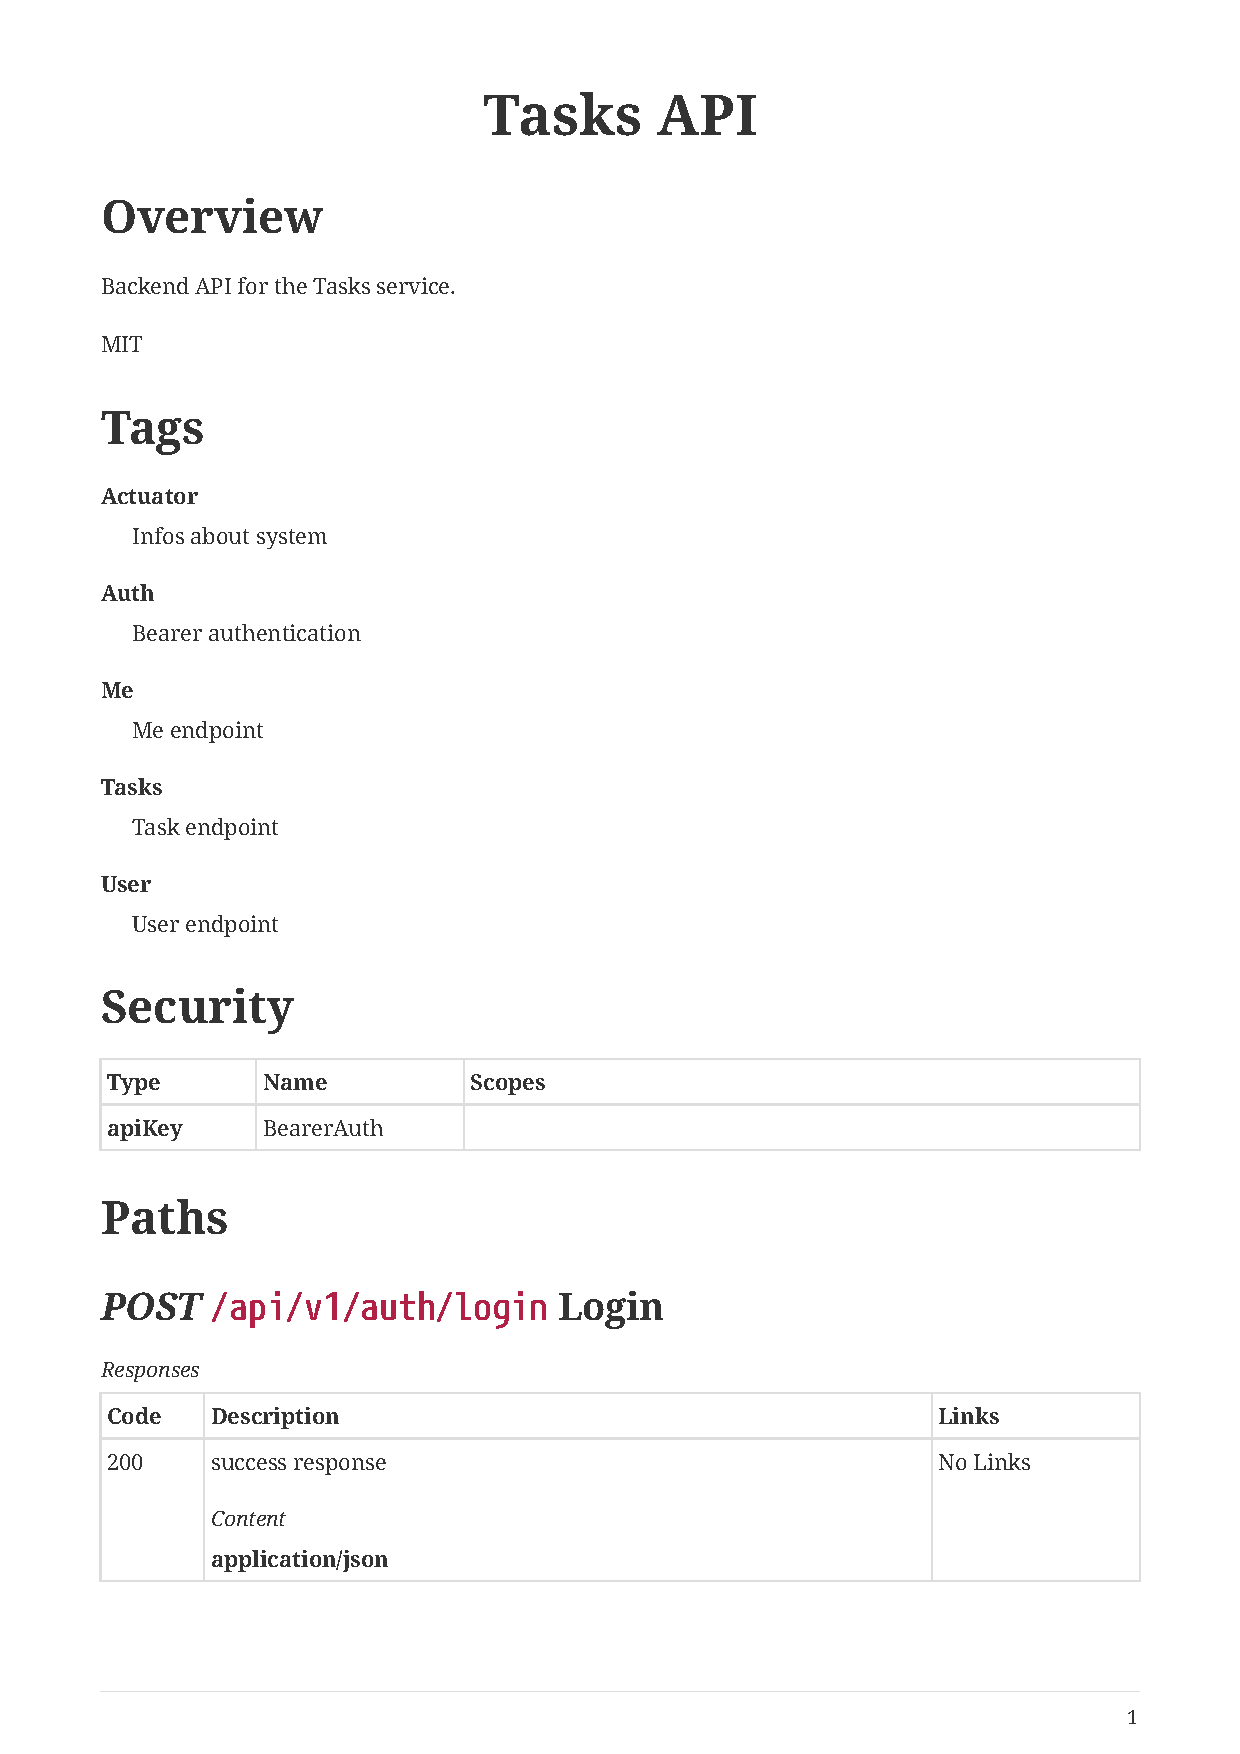
\includepdf[pages=1,scale=.85,pagecommand={\subsection{API Dokumentation}}]{../appendix/swagger_docs.pdf}
    \includepdf[pages=2-,scale=.85,pagecommand={}]{../appendix/swagger_docs.pdf}

    % \begin{figure}[H]
    %     \includegraphics[width=\textwidth]{images/organigram}
    %     \caption{Organigramm Team Pyramid 2021}\label{fig:figure}
    % \end{figure}

\end{document}
